\subsection{Compuertas LSTM y GRU}

Hasta el momento, se ha hecho mención de las salidas $o^{(t)}$ y estados ocultos $h^{(t)}$ solo como
el resultado de operaciones aplicadas por dos funciones; $g$ y $f$ respectivamente. Existen varias
alternativas de construir una \textit{RNN}, una de las maneras más comunes es usando
\ref{eq:rnn_Ht} y \ref{eq:rnn_Ot}:

\begin{equation}
    h^{(t)} = \phi(x^{(t)} W_{x} + h^{(t-1)} W_h + b)
    \label{eq:rnn_Ht}
\end{equation}

\begin{equation}
    o^{(t)} = x^{(t)} W_{out} + b
    \label{eq:rnn_Ot}
\end{equation}

Donde los parámetros compartidos de la red ahora son descritos por las matrices
$W_x \in \mathbb{R}^{d \times k}$, $W_h \in \mathbb{R}^{k \times k}$ y $
W_{out} \in \mathbb{R}^{k \times q}$ con $k$ como la dimensión del estado oculto, $q$ la dimensión
de las salidas $o^{(t)}$, $b \in \mathbb{R} ^ {1 \times q}$ el parámetro de sesgo y $\phi$ es la
función de activación. De esta manera, los pesos de los parámetros aprendidos en la matriz $W_h$
determinan cómo será usada la información del pasado, codificada en $h^{(t-1)}$. Posteriormente
es incluida a la codificación de la información del tiempo actual $t$ calculada por $W_x$. La figura
\ref{fig:rnn_cell} representa gráficamente la lógica usada para calcular los estados ocultos y las
salidas de la red.


\begin{figure}
\centering
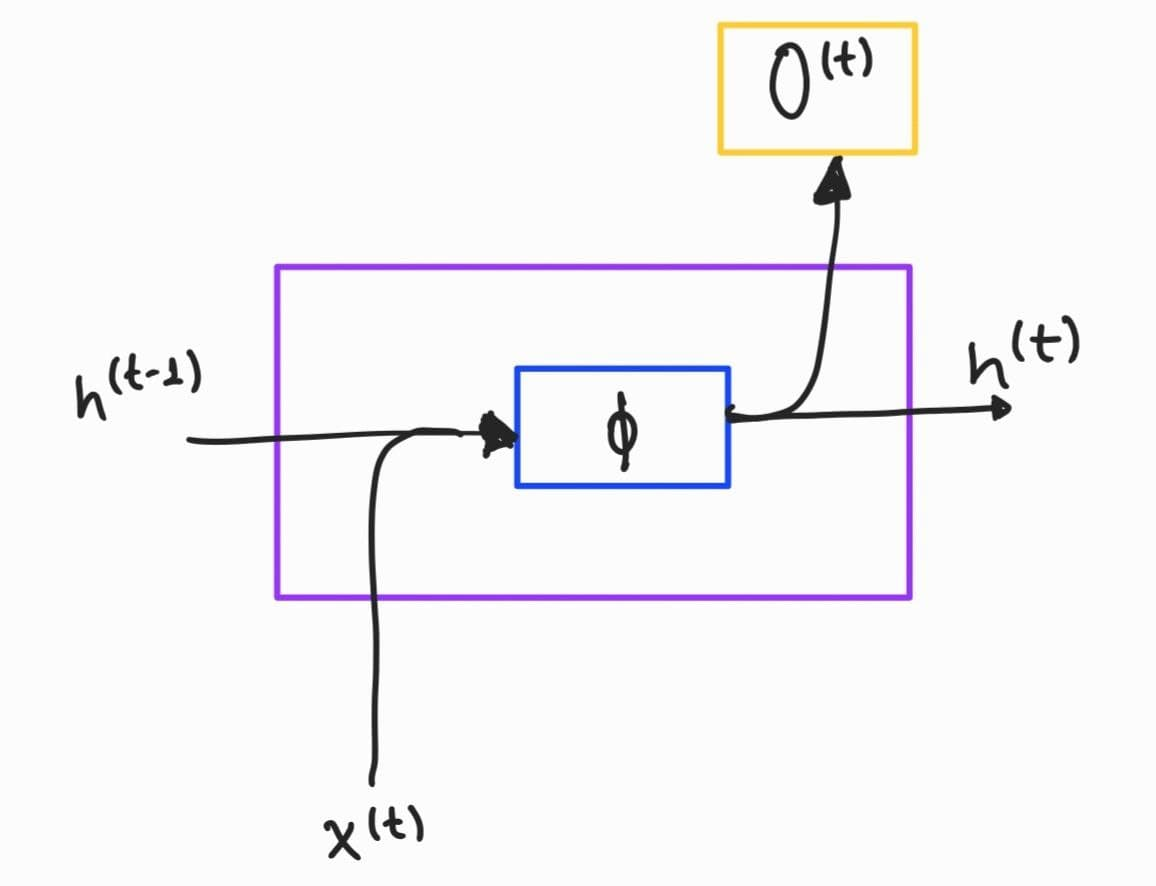
\includegraphics[width=0.4 \textwidth]{Chapters/1. Transformer/Figures/rnn/rnn_cell.jpg}
\caption{Computo del estado oculto y salida de una Red Neuronal Recurrente.}
\label{fig:rnn_cell}
\end{figure}

Sin embargo el cálculo de los estados ocultos mediante \ref{eq:rnn_Ht} presenta algunos problemas.
La interacción entre la información del pasado y la actual siempre es "plana", es decir, la información
fluye a través del tiempo de la misma manera sin forma de dar prioridad o ignorar parte de
esta. Así, resulta una tarea un poco más complicada preservar información relevante a en cada paso
o desechar información que ya no es util para la red. Además mayores problemas de como el
\textit{Desvanecimiento o Explosión del Gradiente} \cite{VanishinGradient}.

% Sección \ref{Vanishing Gradient}

Describir mencionar Vanishing gradiente al hacer multiplicaciones seguidas
mencionar que queremos una forma de acarrear información y desechar la que no sirve
Gated recurren units
